\part{Computer graphics}
\frame{\partpage}

\begin{frame}{What is computer graphics?}
	\begin{itemize}
		\pause\item The process of representing 3D virtual objects on a screen.
		\pause\item "The creation of, manipulation of, analysis of, and interaction with pictorial representations of objects and data using computers." \textit{-- Dictionary of Computing}
		\pause\item Trying to make it look as convincing and/or interesting as possible:
		\begin{itemize}
			\pause\item Shape representation - \textbf{modelling}
			\pause\item How light interacts with the surface - \textbf{shading}
			\begin{itemize}
				\pause\item (Photo)realistic vs. stylised, e.g. cel shading
			\end{itemize}
			\pause\item How light travels around the scene - \textbf{rendering}
		\end{itemize}
	\end{itemize}
\end{frame}

\begin{frame}{Modelling}
	\begin{columns}
		\begin{column}{0.3\textwidth}
			\begin{figure}
				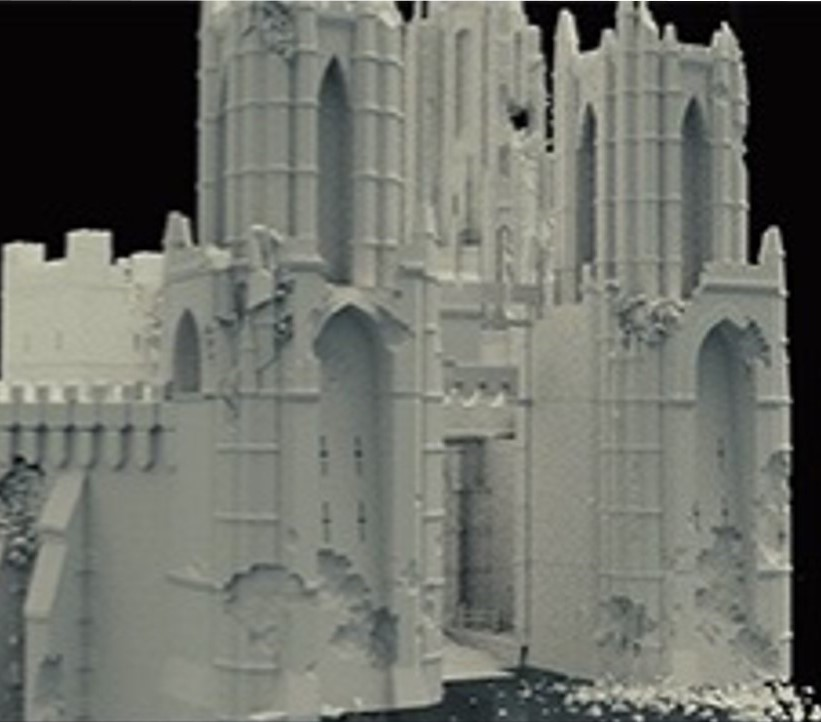
\includegraphics[width=\textwidth]{castle_model}
				\caption*{Image courtesy of \href{https://www.framestore.com}{Framestore}}
			\end{figure}
		\end{column}
		\begin{column}{0.65\textwidth}
			\begin{itemize}
				\pause\item Defines the outline/shape of an object, usually by identifying points or \textbf{vertices} on its surface
				\pause\item Vertices can be generated by an artist using a 3D modelling package, or may be generated procedurally
				\pause\item More vertices => more accurate shape => more data and longer processing times
				\pause\item Algorithms can be used to reduce model complexity without compromising appearance
			\end{itemize}
		\end{column}
	\end{columns}
\end{frame}

\begin{frame}{Shading and rendering}
	\begin{columns}
		\begin{column}{0.3\textwidth}
			\begin{figure}
				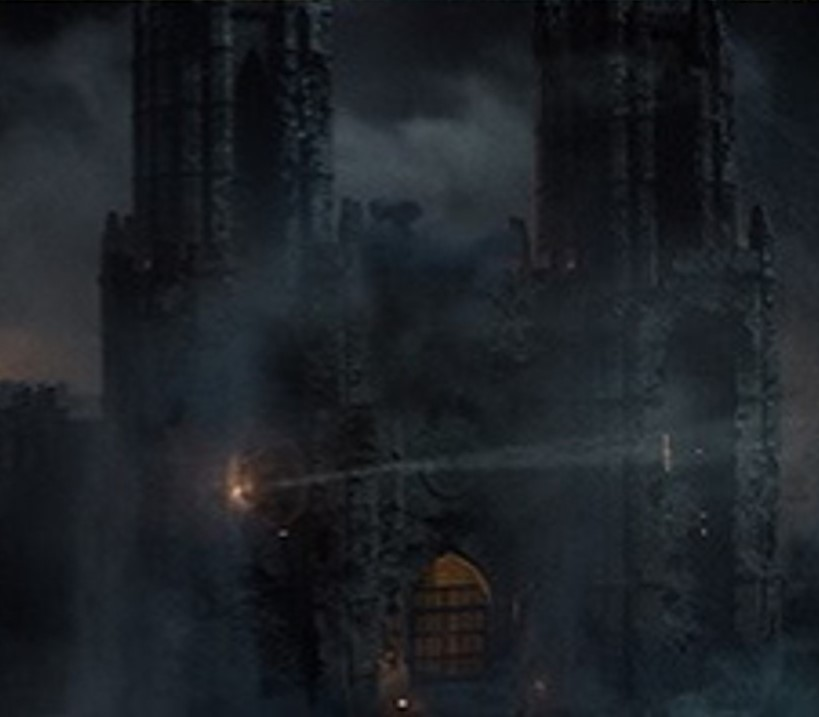
\includegraphics[width=\textwidth]{castle_render}
				\caption*{Image courtesy of \href{https://www.framestore.com}{Framestore}}
			\end{figure}
		\end{column}
		\begin{column}{0.65\textwidth}
			\begin{itemize}
				\pause\item Models are given \textbf{textures} and other surface properties as \textbf{materials}
				\pause\item Use equations from physics to define how light behaves and interacts with materials
				\pause\item A variety of simplifications exist that approximate (some of) the full equation, e.g. Phong shading
			\end{itemize}
		\end{column}
	\end{columns}
\end{frame}